\documentclass[11pt,a4paper]{article}
%\usepackage{fullpage}	% Bigger pages
\usepackage{cite} 		% Include citations
\usepackage{hyperref} 	% Hyperlinks everywhere!
\usepackage{natbib}		% Include bibliography
\usepackage{graphicx}	% Include pictures
\usepackage{amsmath}	% Use \eqref

\begin{document}

\title{Constraining the Hemispherical Structure in the Hidden Layer At the Top of the Earth's Inner Core}
\author{Candidate Number: \\  \\ Supervisor: Prof. Keith Priestley}
\maketitle

\begin{abstract}
Since its discovery in 1936, the Earth's inner core has been well documented by both body wave and normal mode studies. However, one area where properties are not yet well measured is the top of the inner core. The upper region of the inner core is of particular interest as it is thought that as the outer core freezes onto the inner core the variable environment at this boundary is encoded in the properties of the frozen material. 
\end{abstract}

\tableofcontents

\newpage
\section{Introduction}
The inner core was first discovered by Inge Lehmann in 1936, who used the existence of P wave arrivals within the P wave shadow zone to infer a solid-liquid boundary lying within the core mantle boundary (\cite{Lehmann}). Over the following 80 years large progress has been made on measuring the properties of the inner core, but there is much still to learn.

Of particular interest is the velocity and attenuation structure, which can be used to infer the chemical and physical properties of the inner core's constituent material. The following gives a summary of these properties, and is quoted directly from \cite{Deuss2014}:
\begin{itemize}
	\item The top 60-80 km of the inner core is isotropic, and the deeper parts have 3-4\% anisotropy. The anisotropy exists in both velocity and attenuation; waves traveling in the polar direction are faster and more attenuated than waves traveling equatorially.
	\item There may be an innermost inner core with different anisotropy, though evidence is not compelling.\footnote{Research published since \cite{Deuss2014} provides strong evidence for this (\cite{Wang2015}).}
	\item The inner core displays a hemispherical variation: The western hemisphere is more strongly anisotropic, has a lower isotropic compressional velocity, and is less attenuating than the eastern hemisphere. There are sharp boundaries between the two hemispheres.
	\item Inner core superrotation is less than $0.5^{\circ}$ /yr and may even be as small as $0.1-1^{\circ}$ /Myr.
\end{itemize}

The upper inner core is of particular interest, as material from the outer core is currently freezing onto it at a rate of around 1mm/year (\cite{Labrosse2001}). Modelling performed by \cite{Deguen2009a} shows that the velocity structure of the upper inner core should reflect recent processes in the lower upper core. Thus measuring the structure of the upper inner core could in turn give insights into areas such as how the outer core generates the Earth's magnetic field. 

So far only large scale velocity structures have been measured, with the most recent velocity models BEING VERY COARSE GRAINED. In addition the extent to which the methodology used here and elsewhere is not well understood. In this paper we tackle both of these problems.

We do so by taking individual earthquakes that travel to multiple seismic stations and identifying the arrival of distant seismic phases in seismograms. We constrain our analysis to the uppermost inner core as far as is possible, and area not yet investigated in published literature.

Section \ref{sec:Theory} gives an brief theoretical background, with section \ref{sec:Data} describing our data collection and pre-processing. Waveform analysis is discussed in section \ref{sec:Waveforms} leading to regional velocity model results presented in section \ref{sec:Models}.

%%%
\section{Theoretical Background}
\label{sec:Theory}
We use seismic body wave analysis in order to investigate the velocity structure of the upper inner core. These waves elastic waves, caused by earthquakes, that travel through the interior of the Earth.

\subsection{Body Wave Theory}
Here we summarise the main aspects of seismic body wave theory, taken from \cite{Shearer2009}.

Under the assumptions of a continuous, linearly elastic medium, infinitesimal strains and constant medium properties one can derive the elastic wave equation
\begin{equation}
	\rho \frac{\partial^{2} \vec{u}}{\partial t^{2}} = \left ( \lambda + \mu \right ) \nabla \left ( \nabla \cdot \vec{u} \right ) + \mu \nabla^{2} \vec{u}
	\label{eq:Wave Equation}
\end{equation}
where u is the local displacement vector, $\rho$ the density of the medium and $\lambda$ and $\mu$  Lam\'{e} parameters of the medium. A general displacement vector can be decomposed into irrotational scalar and solenoidal vector potentials such that
\begin{equation}
	u \equiv \nabla \phi + \nabla \times \vec{\psi}
	\label{eq:Displacement}
\end{equation}
Substituting \eqref{eq:Displacement} in to \eqref{eq:Wave Equation} yields two independent wave equations, one for $\phi$ and one for $\vec{\psi}$, which describe P-waves and S-waves respectively. P-waves are compressional with displacements occurring parallel to the wave vector, whereas S-waves are transverse with displacements occurring perpendicular to the wave vector. These wave equations take the form
\begin{equation}
	\frac{\partial^{2} \phi}{\partial t^{2}} = c^{2} \left ( \vec{x} \right ) \nabla^{2} \phi
\end{equation}
where $c(\vec{x})$ is the local wave velocity that depends on position. A velocity model is a full specification of $c(\vec{x})$ in the region of interest.

\subsection{Sampling the Inner Core}
Because the outer core is liquid with $\mu \approx 0$ and thus does not transmit S-waves, it is P-waves that are used to sample the inner core. Figure PUT FIGURE HERE shows the ray path for the PKiKP and PKIKP phase; they travel almost identical paths through the Crust, Mantle and upper Outer Core, after which PKiKP reflects off the Inner Core boundary, whereas PKIKP travels just underneath the boundary in the Inner Core.

All measurements are compared to the radially symmetric AK135 global velocity model (\cite{Kennett1995b}), from which we seek to measure perturbations about. The residual travel time CHECK ME is defined after \cite{Waszek2011a} as
\begin{equation}
	\delta t = \left ( t_{PKiKP} - t_{PKIKP} \right )_{observed} -  \left ( t_{PKiKP} - t_{PKIKP} \right )_{model}
\end{equation}
This equation can be reformulated as an integral along the ray paths
\begin{equation}
		\delta t = \left (  \int \frac{1}{v_{obs}} - \frac{1}{v_{model}} ds  \right )_{PKiKP} - \left (  \int \frac{1}{v_{obs}} - \frac{1}{v_{model}} ds \right )_{PKIKP}
		\label{eq:deltat}
\end{equation}
where the path to be integrated along is indicated by the subscript outside the brackets, and in general the velocities vary as a function of position.

Taking $v_{obs} = v_{model} + \delta v$ gives
\begin{equation}
	\delta t = \int \frac{\delta v}{v^{2}_{model}} ds
\end{equation}

For depths below the Inner Core boundary of less than 50km $v_{model}$ is constant and we assume $\delta v$ is also a constant such that we are measuring only the average velocity perturbation along the ray path. We are thus left with the equation that will allow us to compute $\delta v$
\begin{equation}
	\delta v = \frac{\delta t}{t} v_{model}
\end{equation}
where $t$ is the time PKIKP spends in the inner core. If instead we wish to calculate a layered model, we simply apply the above results to the uppermost layer, and then take the effect of the new layer into account when calculating the properties of subsequent layers.

%%%
\section{Data Selection}
\label{sec:Data}
We present regional velocity models, derived from INSERT NUMBER HERE earthquakes. The datasets are selected to meet the following criteria:

\begin{itemize}
	\item An epicentral distance of $115^{\circ}$ - $135^{\circ}$ from the earthquake covers the majority of North America, where there is the highest worldwide density of seismograms.
	\item A hypo centre greater than 15km, to minimise possible interference between PKIKP (PKiKP) and pPKIKP (pPKiKP) waves.
	\item A magnitude greater than 5.3 and less than 6.3 to ensure a large enough earthquake to produce an observable signal, whilst a small enough earthquake such that the rupture mechanism is likely to be impulsive.
	\item A fracture mechanism that is primarily dip slip (as opposed to strike slip). As the ray paths are nearly vertical when they reach the seismic stations, we require significant amounts of energy to be focused in the vertical direction at the site of the earthquake.
	\item Data is selected for a $30^{\circ}$ azimuthal range in order to only construct a small regional velocity model.
\end{itemize}

Each seismogram is filtered between 0.7Hz - 2Hz in order to focus on the expected frequency of $\sim$1Hz whilst removing unwanted noise. Individual seismograms are checked by hand, and only those showing a clear PKiKP signal near the predicted arrival time are kept for further analysis.

%%%
\section{Waveform Analysis}
\label{sec:Waveforms}
The same analysis was performed on each individual event, allowing construction of a detailed velocity model for several CHANGE ME regions. Here we describe the analysis performed using the specific example of the Celebes Sea earthquake that occurred on 2014/04/16.\footnote{For a complete listing of all events and associated parameters see Appendix \ref{App:Event listing}.}

Synthetic waveforms are computed using the WKBJ ray tracing program (\cite{Chapman1976}), and predicted ray paths and travel times computed using the TauP toolkit (\cite{Crotwell1999}). Initial plots are shown for both real and synthetic data in figures \ref{fig:Real nonaligned} and \ref{fig:Synth nonaligned} respectively, with zero time occurring at the time of the earthquake, taken from the global CMT catalogue (\cite{Dziewonski1981}, \cite{Alboussiere2012}). Overplotted are theoretical PKIKP and PKiKP travel times computed using the AK135 model (\cite{Kennett1995b}). The predicted travel times agree well with the data in both cases. For shorter epicentral distances the predicted arrival time become closer, suggesting that eventually there will be a minimum distance at which the two phases will be observable. In the next subsection we attempt to quantify this minimum distance.

\begin{figure}
	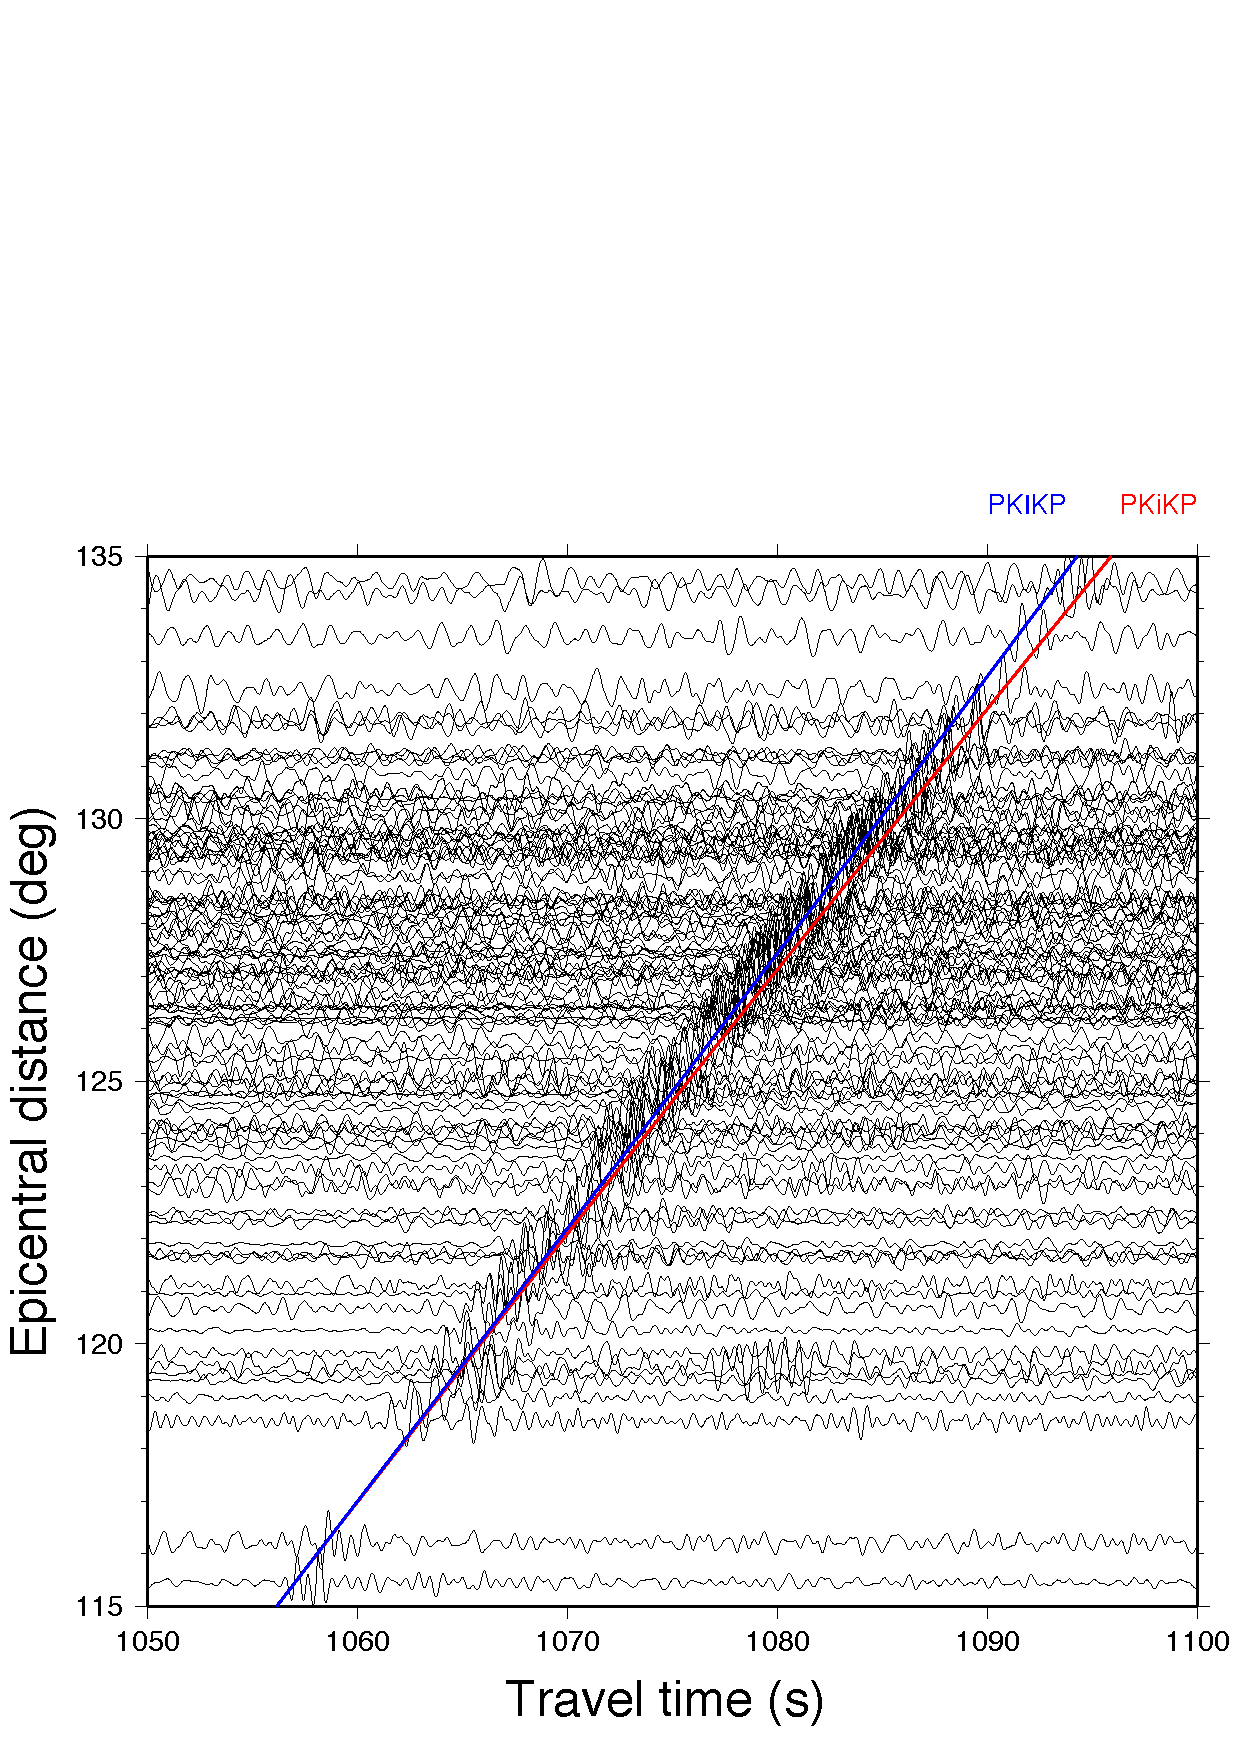
\includegraphics[width=\textwidth]{figures/celebessea_real.pdf}
	\caption{Real seismogram data from the Celebes Sea event after clear event selection. Each seismogram is zeroed on the earthquake time. Over plotted lines are theoretical phase arrivals computed using the AK135 model.}
	\label{fig:Real nonaligned}
\end{figure}

\begin{figure}
	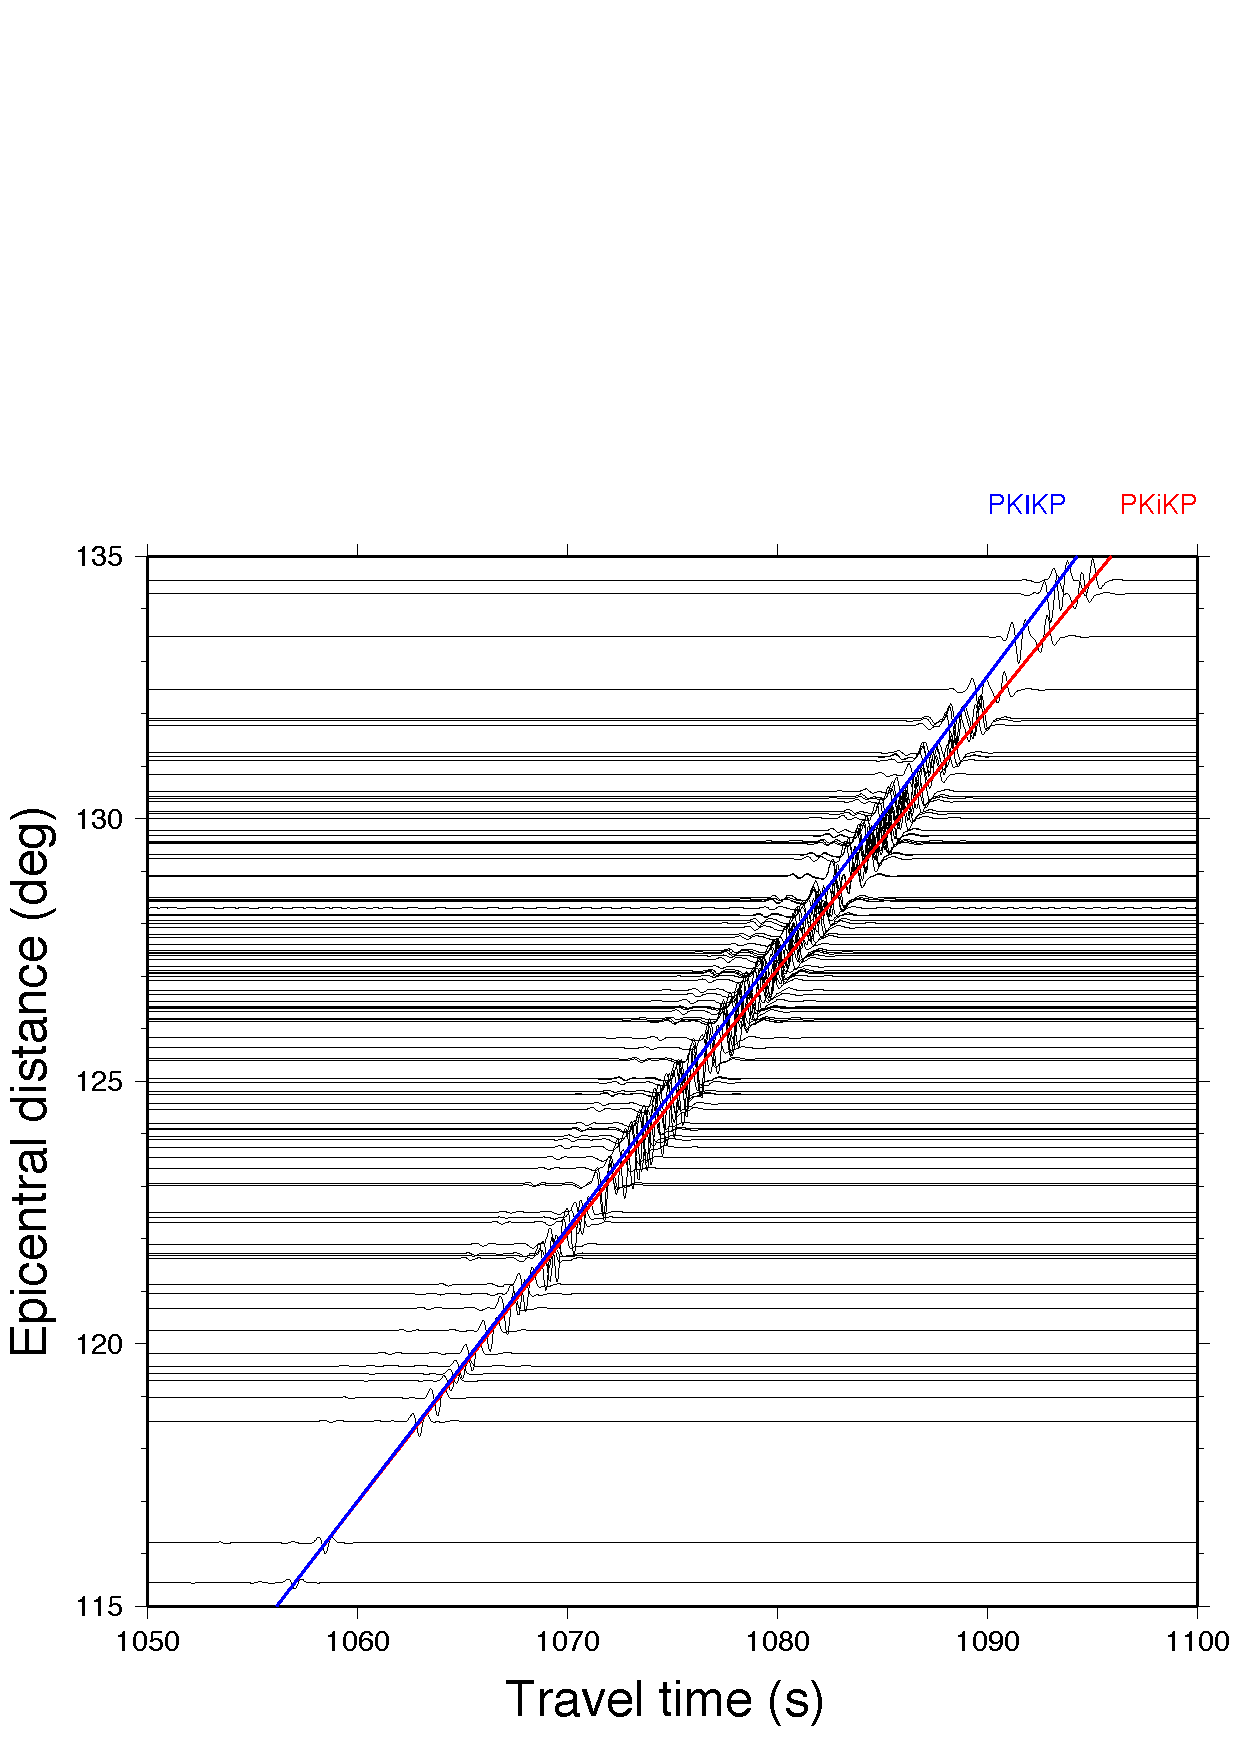
\includegraphics[width=\textwidth]{figures/celebessea_synthetic_both.pdf}
	\caption{Synthetic seismogram data for the Celebes Sea event.. Each seismogram is zeroed on the earthquake time. Over plotted lines show theoretical phase arrivals computed using the AK135 model.}
	\label{fig:Synth nonaligned}
\end{figure}

\subsection{Quantifying minimum resolvable depth}
In order to see more clearly the contributions of the individual phases to the overall seismogram we plot individual PKIKP and PKiKP synthetics, and align them to the final large upswing of the PKiKP phase. Figure \ref{fig:Synth aligned} shows the results of this analysis. At smaller epicentral distances PKIKP gets weaker and PKiKP develops a large upswing to the left. Both of these features could mean that when measuring the peak to peak difference at low distances on the combined seismogram (or equivalently the real data) we are measuring two features of PKiKP and not one feature from each phase. This criterial will be met either when PKIKP differences are larger than combined differences, or when PKiKP and combined differences coincide.

\begin{figure}
	\centering
	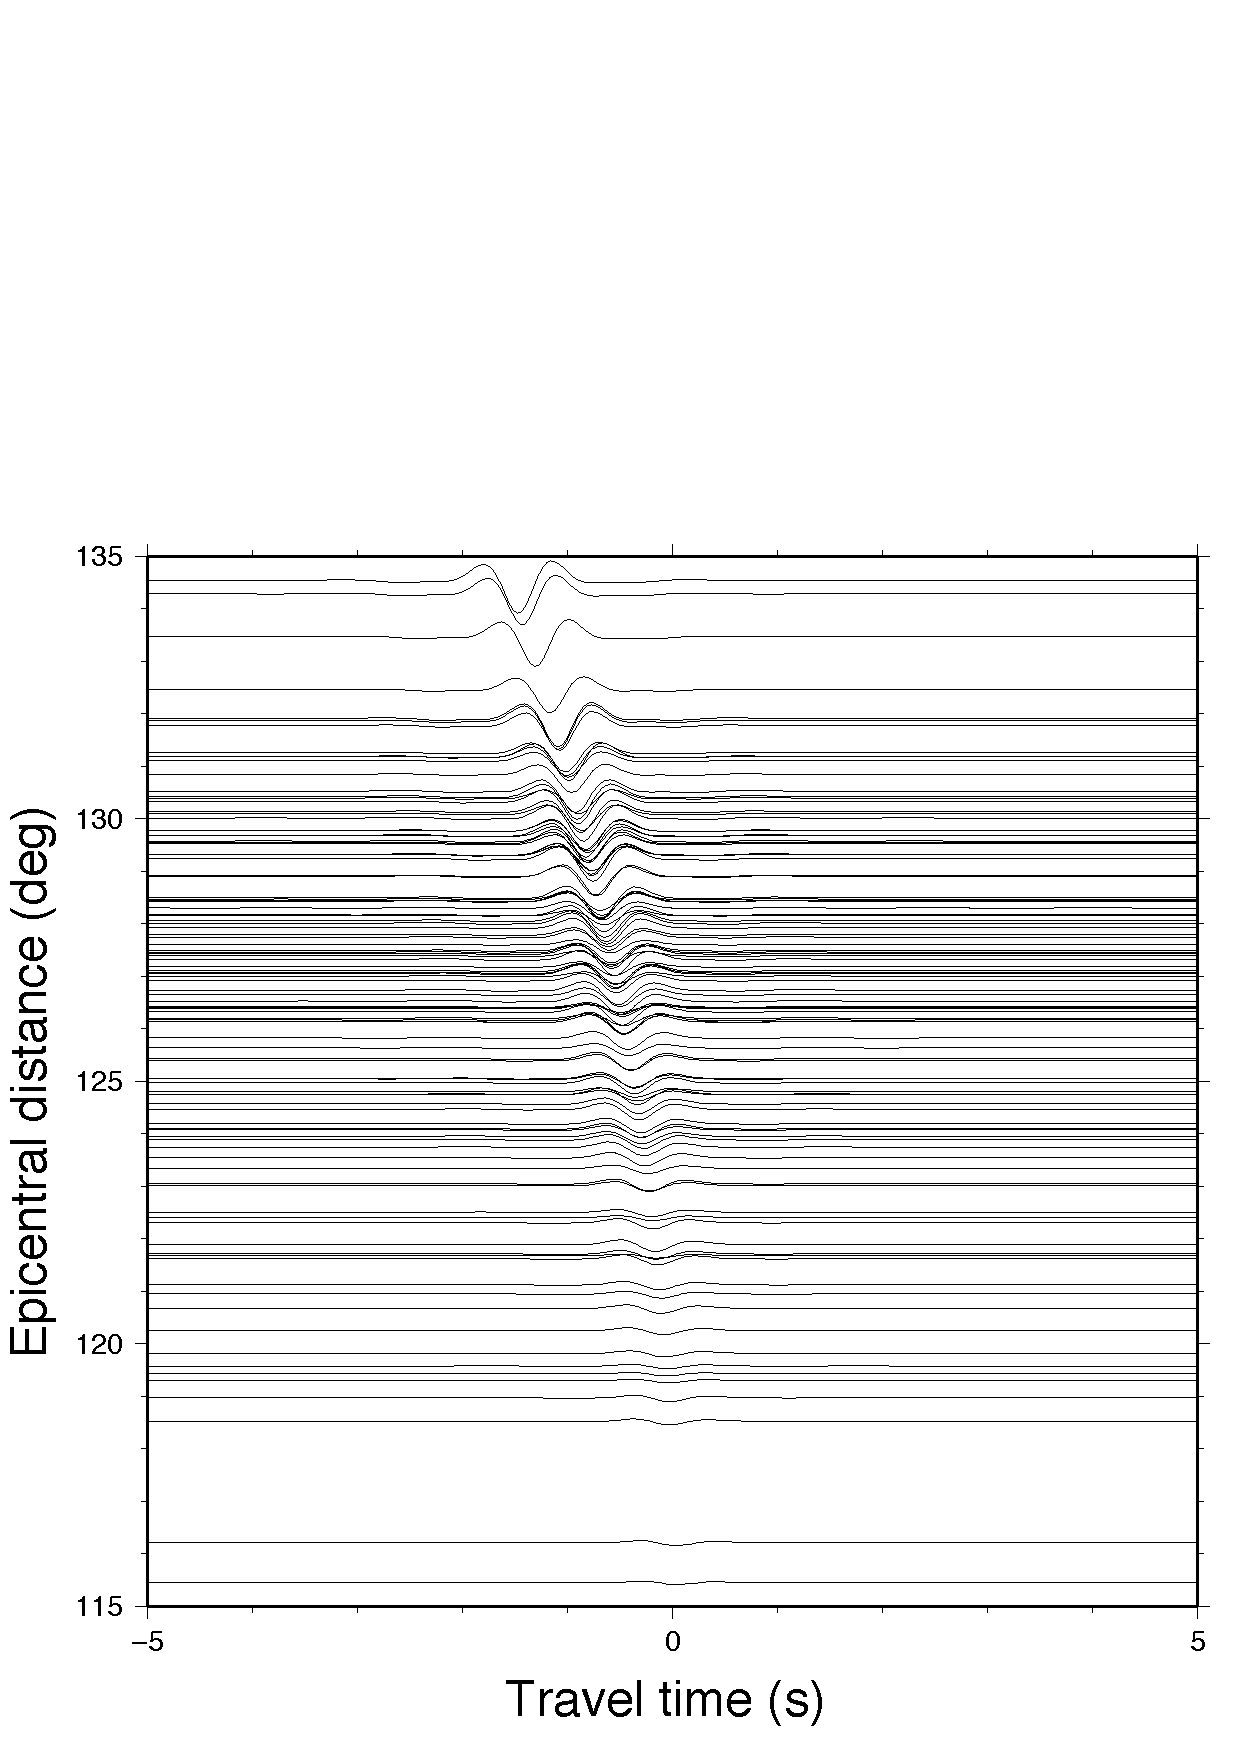
\includegraphics[width=0.49\textwidth]{figures/celebessea_KIK_aligned}
	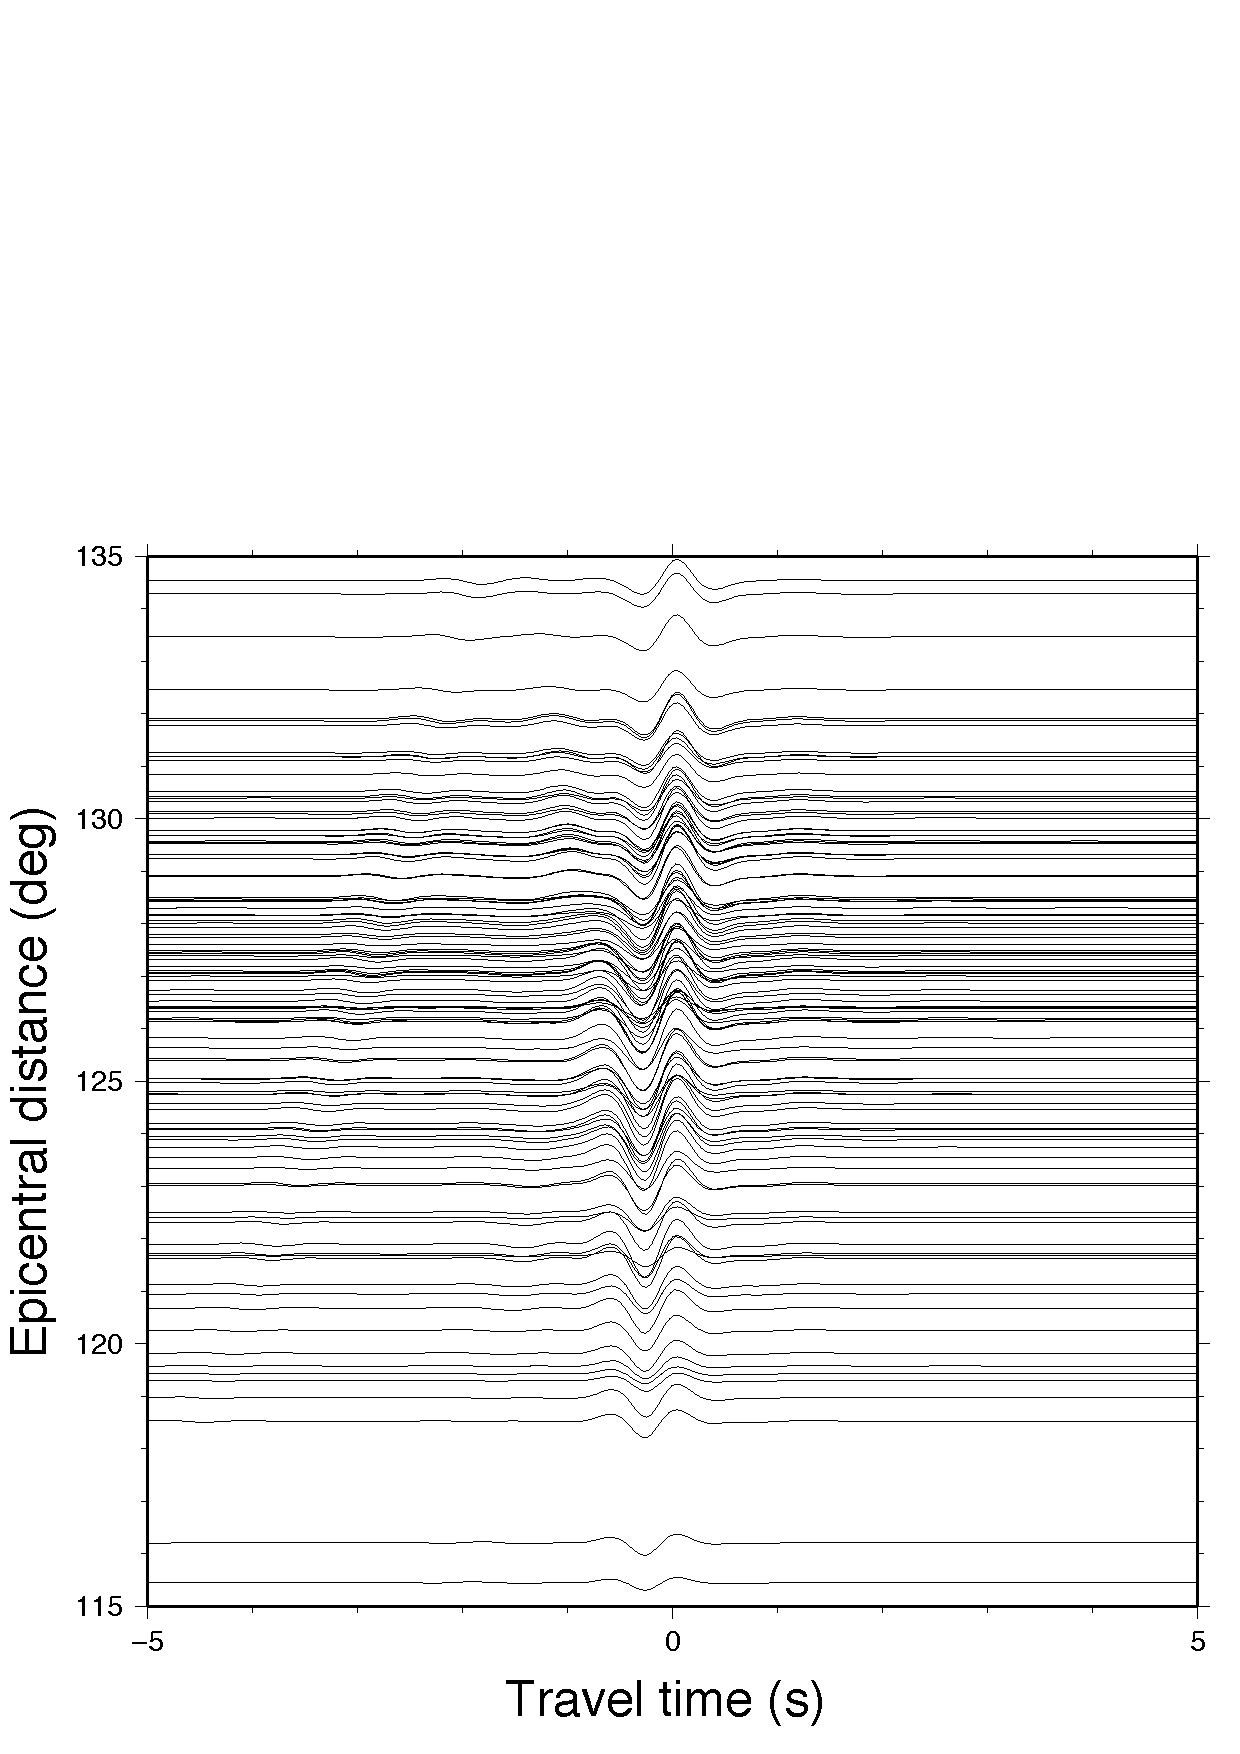
\includegraphics[width=0.49\textwidth]{figures/celebessea_pkikp_aligned}
	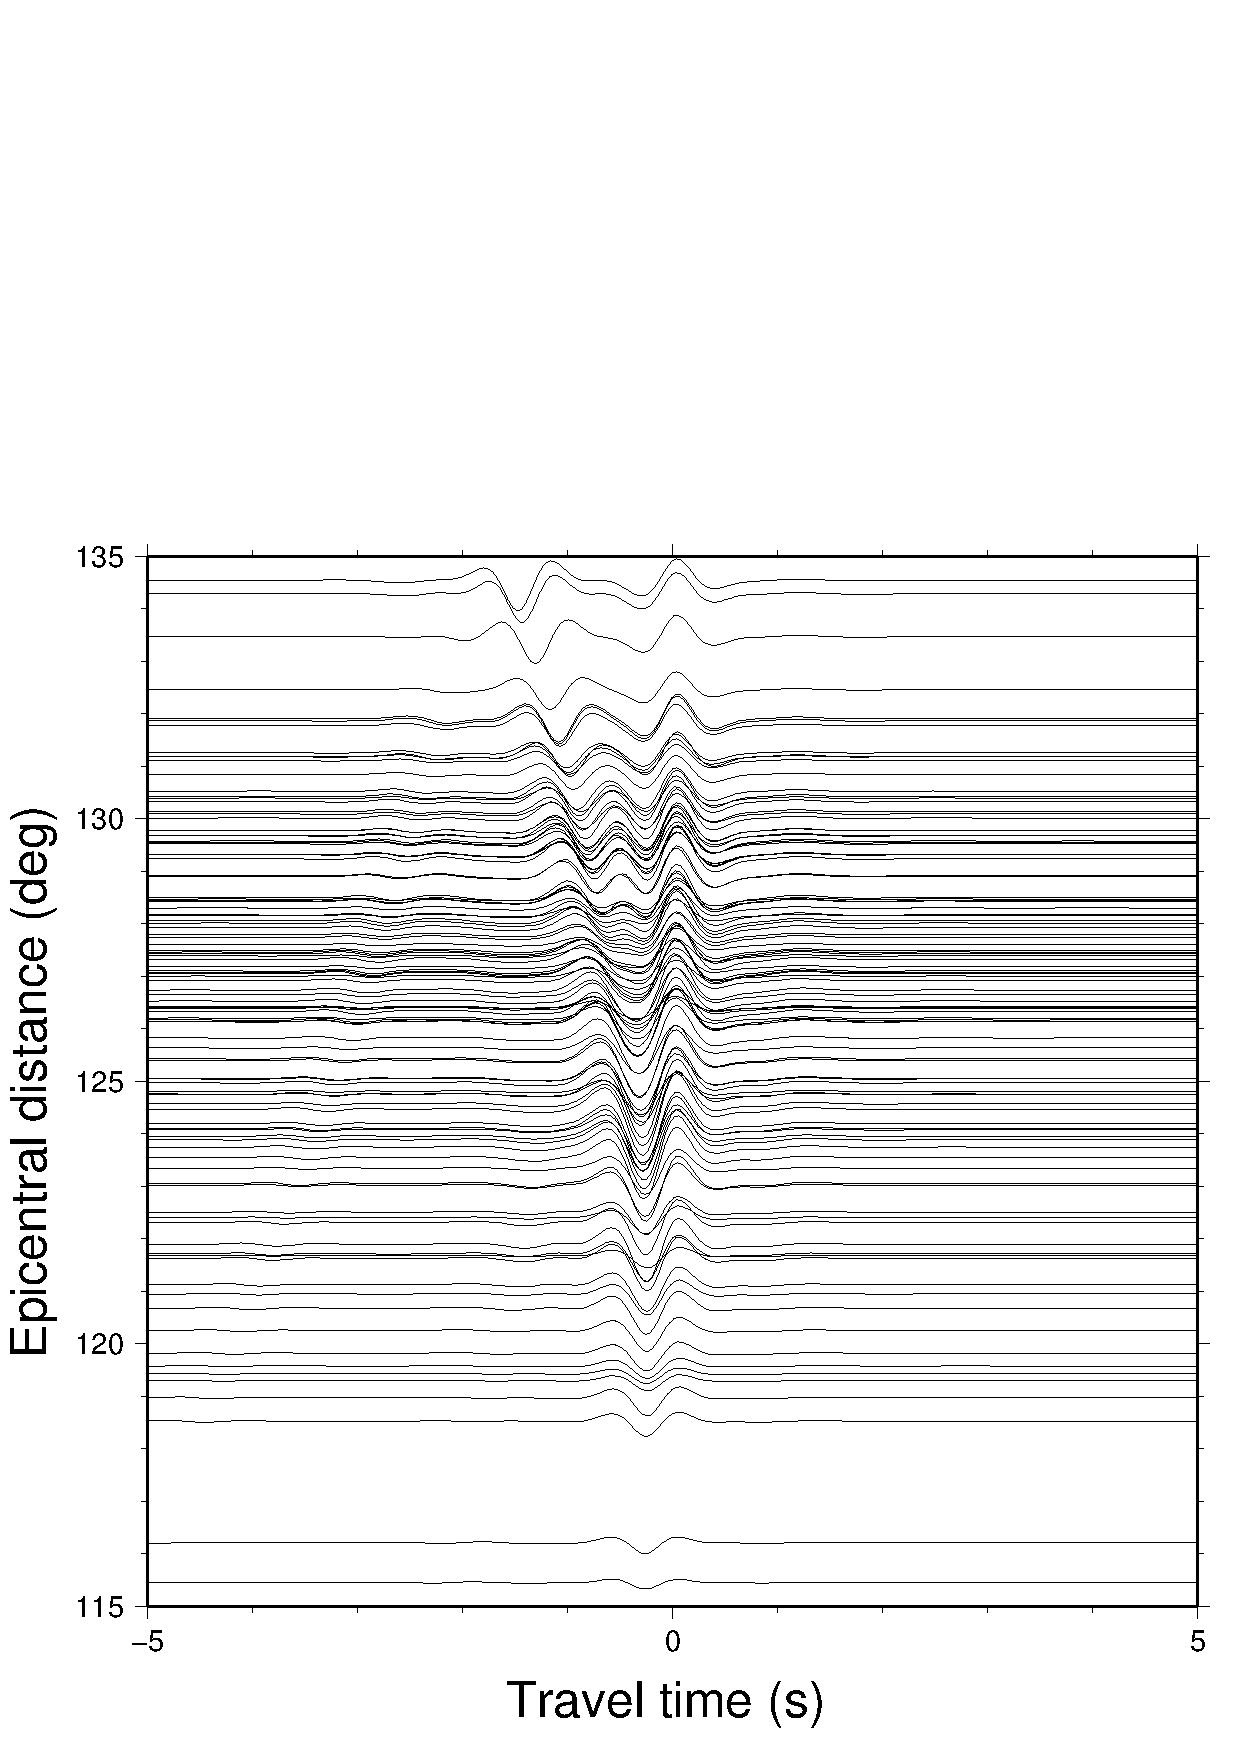
\includegraphics[width=0.49\textwidth]{figures/celebessea_both_aligned}
	\caption{Separated PKIKP (top left) PKiKP (top right), and combined (bottom) synthetic seismograms for the Celebes Sea event.}
	\label{fig:Synth aligned}
\end{figure}

Figure \ref{fig:Min distance} shows measurements of peak to peak differences for PKiKP, PKIKP and combined synthetic waveforms. It can be clearly seen that below $126^{\circ}$ PKiKP and combined measurements coincide, thus setting $126^{\circ}$ as the maximum epicentral distance at which the two phases can be distinguished.

\begin{figure}
	\centering
	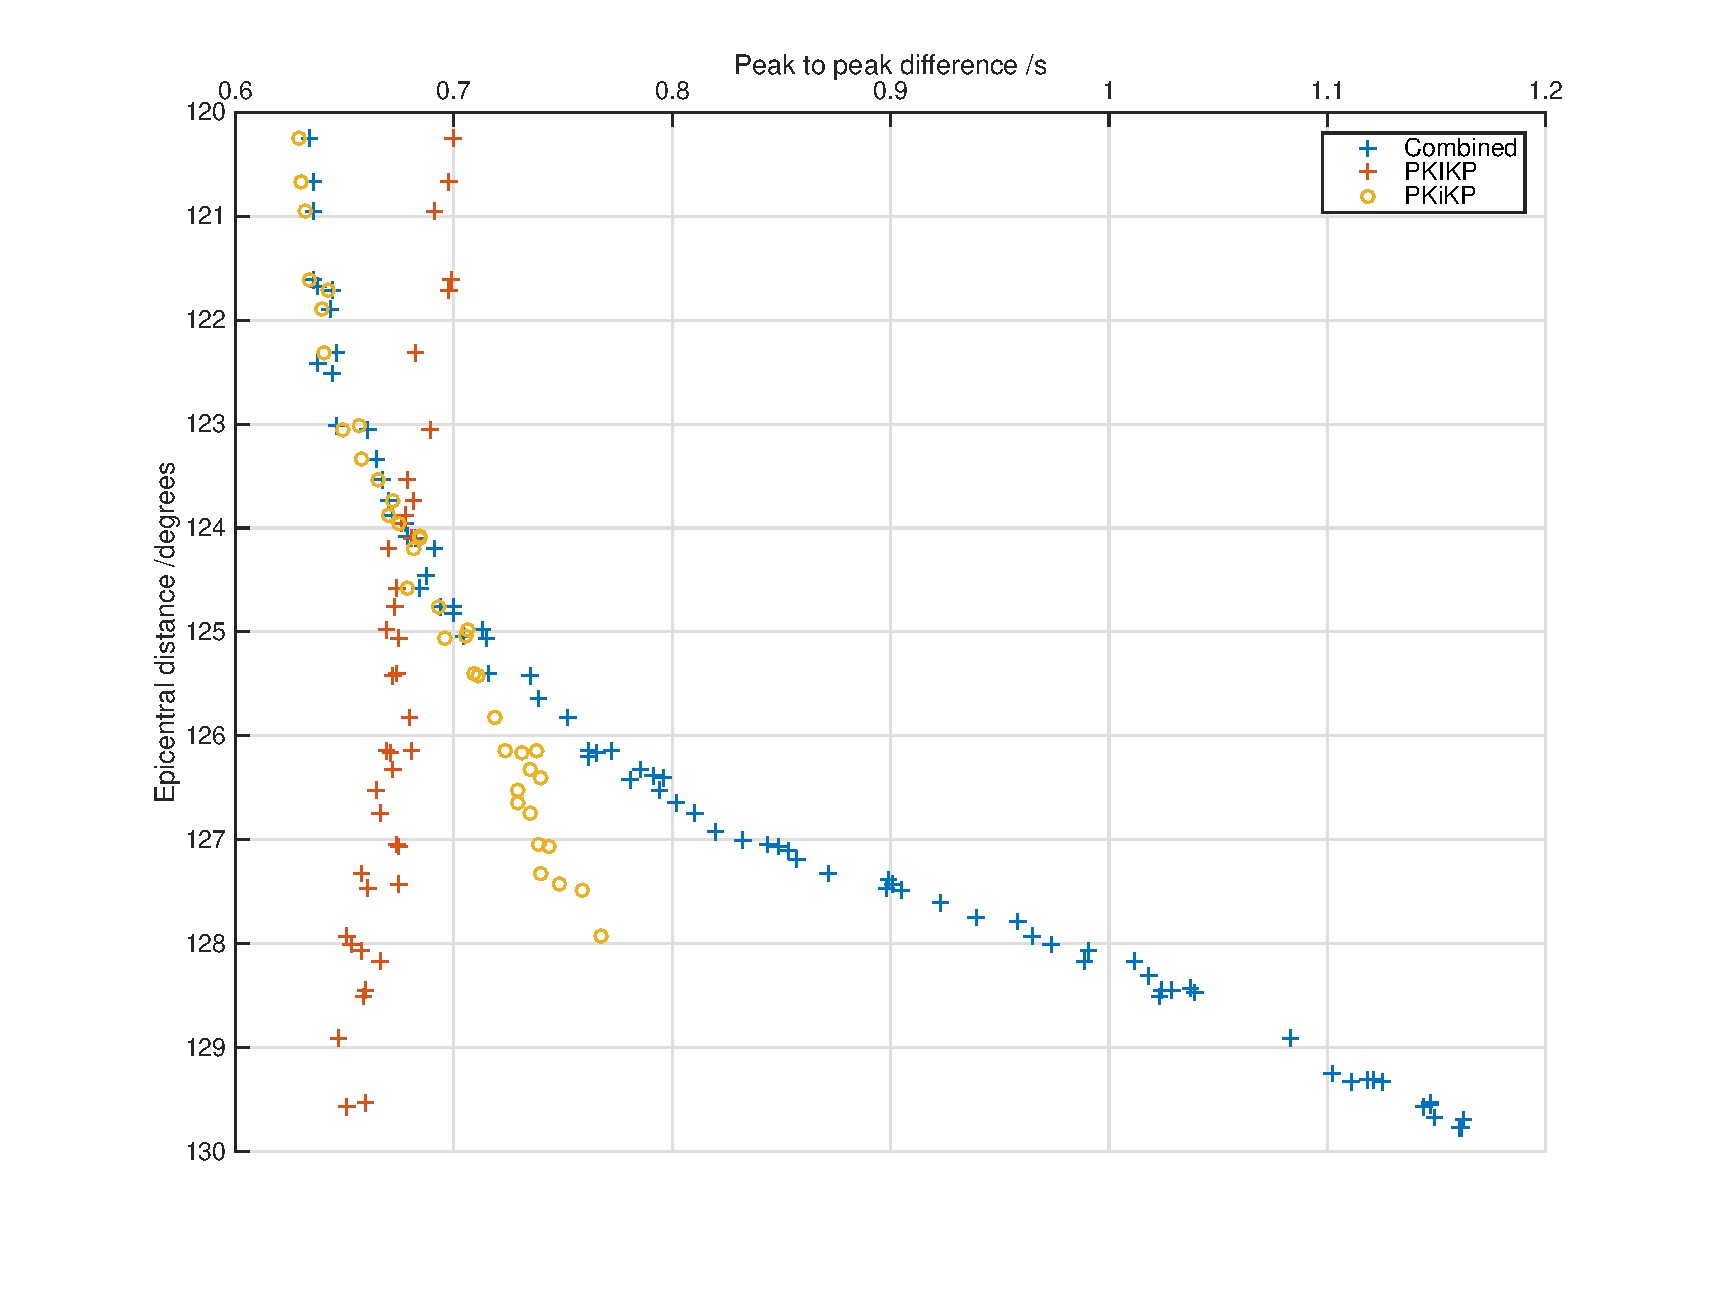
\includegraphics[width=\textwidth]{figures/min_distance}
	\caption{Peak to peak travel times recorded from synthetic data generated for the Celebes Sea earthquake. The difference is taken between the two large upswings in each case.}
	\label{fig:Min distance}
\end{figure}

\section{Updated velocity models}
\label{sec:Models}

\appendix
\section{Event Listing}
\label{App:Event listing}
\begin{tabular}{| l | l | l | l | l | l |}
	\hline Location		& Latitude	& Longitude	& Depth /km	& Date		& Time (GMT) \\
	\hline Celebes Sea	& 4.55	& 122.82		& 575.0		& 2014/04/16	& 4:28:20.0 \\ 
	\hline
\end{tabular}

\section{Aligned Sesimograms}

\section{Residual Plots}

% Bibliography
\bibliographystyle{yahapj}
\bibliography{/Users/dstansby/Physics/Papers/library}

\end{document}